\documentclass[aspectratio=169,11pt]{beamer}
\usetheme{default}
\usecolortheme{default}

\usepackage{tikz}
\usetikzlibrary{shapes,arrows,positioning,fit,backgrounds,calc}
\usepackage{xcolor}
\usepackage{colortbl}
\usepackage{booktabs}
\usepackage{graphicx}
\usepackage{amsmath}

% Custom colors
\definecolor{userblue}{RGB}{25,50,128}
\definecolor{assistgreen}{RGB}{25,100,50}
\definecolor{lightblue}{RGB}{235,240,255}
\definecolor{lightgreen}{RGB}{235,255,240}
\definecolor{lightred}{RGB}{255,240,240}
\definecolor{darkred}{RGB}{150,30,30}
\definecolor{purple}{RGB}{100,75,128}
\definecolor{lightpurple}{RGB}{245,240,250}
\definecolor{orange}{RGB}{128,75,50}
\definecolor{lightorange}{RGB}{255,245,240}

% Remove navigation symbols
\setbeamertemplate{navigation symbols}{}

% Custom title formatting
\setbeamercolor{title}{fg=userblue}
\setbeamercolor{frametitle}{fg=userblue}
\setbeamerfont{frametitle}{size=\large,series=\bfseries}

\title{\textbf{RL Turns Stochastic Parrots into Parrots}}
\subtitle{Evidence for Dual Processing Modes in Instruct LLMs}
\author{Entropy as a signature of processing mode}
\date{}

\begin{document}

% ============== SLIDE 1: Title ==============
\begin{frame}
\titlepage
\end{frame}

% ============== SLIDE 2: Core Hypothesis ==============
\begin{frame}{The Core Hypothesis}

\vspace{0.2cm}
\begin{center}
\fcolorbox{userblue}{lightblue!30}{
\begin{minipage}{0.85\textwidth}
\centering
\large
\textbf{User tokens are processed for \textcolor{userblue}{intent}}\\[0.1cm]
\textbf{Assistant tokens are processed for \textcolor{assistgreen}{execution}}
\end{minipage}
}
\end{center}

\vspace{0.4cm}
\begin{columns}[T]
\begin{column}{0.48\textwidth}
\footnotesize
\fcolorbox{darkred}{lightred}{
\begin{minipage}{0.93\textwidth}
\textbf{\textcolor{darkred}{PREDICTION 1: Entropy Differs by Role}}\\[0.1cm]
Freed from the yoke of predicting an unknown distribution, models should constrain their entropy to gain greater control.
\end{minipage}
}
\vspace{0.15cm}

\fcolorbox{purple}{lightpurple}{
\begin{minipage}{0.93\textwidth}
\textbf{\textcolor{purple}{PREDICTION 3: Assistant Is Pre-Planned}}\\[0.1cm]
Execution mode requires committing to a plan before acting. Models should store intent during user processing and execute against it.
\end{minipage}
}
\end{column}
\begin{column}{0.48\textwidth}
\footnotesize
\fcolorbox{userblue}{lightblue}{
\begin{minipage}{0.93\textwidth}
\textbf{\textcolor{userblue}{PREDICTION 2: Entropy = Confidence}}\\[0.1cm]
Since the token distribution is a distribution over the assistant's actions, entropy should be a measure of confidence.
\end{minipage}
}
\vspace{0.15cm}

\fcolorbox{orange}{lightorange}{
\begin{minipage}{0.93\textwidth}
\textbf{\textcolor{orange}{PREDICTION 4: User Goals Are Stickier}}\\[0.1cm]
The assistant serves the user, not itself. User-stated goals should be defended more strongly than self-stated goals.
\end{minipage}
}
\end{column}
\end{columns}

\end{frame}

% ============== SLIDE 3: Entropy by Role ==============
% DATA SOURCES:
% - OLMo data: olmo3_7b/cache/rlzero/T07/ analyzed by olmo3_7b/scripts/analyze_entropy_by_role.py
% - Llama/Qwen cross-model: llama70b/results/activation_sim/ and qwen72b/results/activation_sim/
\begin{frame}{Entropy by Role}
\small
\textcolor{gray}{\textit{Supports Prediction 1 | Measured from on-policy chat caches with role labels}}

\vspace{0.2cm}
\begin{table}[h]
\centering
\small
\begin{tabular}{l|c|c|c|l}
\toprule
\textbf{Model} & \textbf{User Entropy} & \textbf{Asst Entropy} & \textbf{Ratio} & \textbf{Data Source} \\
\midrule
OLMo 3-7B RLZero & \cellcolor{lightred}2.36 $\pm$ 2.71 & \cellcolor{lightgreen}0.73 $\pm$ 1.48 & 3.2x & rlzero/T07 cache \\  % olmo3_7b/results/entropy_by_role/
Llama 3.1 70B Instruct & \cellcolor{lightred}1.39 $\pm$ 1.08 & \cellcolor{lightgreen}0.39 $\pm$ 0.52 & 3.6x & activation\_sim \\  % llama70b/results/activation_sim/
Qwen 2.5 72B Instruct & \cellcolor{lightred}0.80 $\pm$ 0.96 & \cellcolor{lightgreen}0.29 $\pm$ 0.42 & 2.8x & activation\_sim \\  % qwen72b/results/activation_sim/
\bottomrule
\end{tabular}
\end{table}

\vspace{0.2cm}
\textbf{OLMo 3-7B Entropy by Condition:}
\begin{table}[h]
\centering
\small
\begin{tabular}{l|c|c}
\toprule
\textbf{Condition} & \textbf{Entropy (nats)} & \textbf{N tokens} \\
\midrule
Base model on C4 & 1.98 $\pm$ 1.77 & 29,632 \\
RLZero User (problem) & \cellcolor{lightred}2.36 $\pm$ 2.71 & 2,822 \\
RLZero Assistant (reasoning) & \cellcolor{lightgreen}0.73 $\pm$ 1.48 & 20,480 \\
\bottomrule
\end{tabular}
\end{table}

\begin{itemize}
\item User entropy 3-4x higher than assistant across all models tested
\item Base model on C4: 1.98 nats --- between user and assistant entropy
\item Consistent pattern across OLMo, Llama, and Qwen families
\end{itemize}

\end{frame}

% ============== SLIDE 4: Role Tags Effect ==============
% DATA SOURCES:
% - GPT-OSS role tag effect: gptoss_20b/results/role_tag_entropy/ analyzed by gptoss_20b/scripts/measure_role_tag_effect.py
% - Cross-model entropy: llama70b/results/activation_sim/ and qwen72b/results/activation_sim/
\begin{frame}{Role Tags Reduce Entropy on Random Text}
\small
\textcolor{gray}{\textit{Supports Prediction 1 | Assistant role markers reduce entropy even on OFF-POLICY text}}

\vspace{0.15cm}
\textbf{Role Tag Effect on Same Text} (GPT-OSS 20B model)  % gptoss_20b/results/role_tag_entropy/

\begin{table}[h]
\centering
\footnotesize
\begin{tabular}{l|c|c|c|c}
\toprule
\textbf{Text Type} & \textbf{As User} & \textbf{As Assistant} & \textbf{Effect ($\Delta$)} & \textbf{\% Reduction} \\
\midrule
Base/web text (C4, off-policy) & \cellcolor{lightred}5.14 $\pm$ 0.59 & \cellcolor{lightgreen}3.72 $\pm$ 0.96 & -1.42 nats & 28\% \\
Assistant responses (on-policy) & \cellcolor{lightred}2.90 $\pm$ 0.70 & \cellcolor{lightgreen}1.56 $\pm$ 0.42 & -1.34 nats & 46\% \\
CoT reasoning text & 1.35 $\pm$ 0.35 & 1.32 $\pm$ 0.24 & -0.03 nats & 2\% \\
\bottomrule
\end{tabular}
\end{table}

\vspace{0.1cm}
\textbf{Cross-Model Entropy} (Llama 70B + Qwen 72B)
\begin{table}[h]
\centering
\footnotesize
\begin{tabular}{l|c|c|l}
\toprule
\textbf{Text Author $\rightarrow$} & \textbf{Llama Text} & \textbf{Qwen Text} & \textbf{Self-Preference} \\
\midrule
Llama evaluator & \cellcolor{lightgreen}0.363 & 0.728 & 2.0x lower on own \\
Qwen evaluator & 0.438 & \cellcolor{lightgreen}0.312 & 1.4x lower on own \\
\bottomrule
\end{tabular}
\end{table}

\begin{itemize}\itemsep0pt
\item \textbf{Key finding:} Assistant role tags reduce entropy 28\% on RANDOM WEB TEXT
\item Effect is larger on assistant-style text (46\%) than on CoT reasoning (2\%)
\item Models have lower entropy on their OWN outputs vs other models' outputs
\item This shows role markers activate `execution mode' even on off-policy text
\end{itemize}

\end{frame}

% ============== SLIDE 5: Entropy Manifolds ==============
% DATA SOURCES (images):
% - Llama 8B Base: llama31_8b/results/base_entropy_centroids_pc1_pc2.png
% - Llama 70B Instruct: llama70b/results/entropy_centroids/entropy_manifolds_by_layer.png
% - OLMo Base: olmo3_7b/results/entropy_centroids/base-on-base.png
% - OLMo Chat: olmo3_7b/results/entropy_centroids/rlzero-chat.png
\begin{frame}{Different Entropy Manifolds}
\small
\textcolor{gray}{\textit{Supports Prediction 2 | Base models: wide range. On-policy generation: compressed manifold}}

\vspace{0.1cm}
\begin{columns}[T]
\begin{column}{0.48\textwidth}
\centering
\textbf{Llama 8B BASE}\\
\vspace{0.05cm}
\includegraphics[width=0.95\textwidth,height=2.8cm,keepaspectratio]{llama31_8b/results/base_entropy_centroids_pc1_pc2.png}
\end{column}
\begin{column}{0.48\textwidth}
\centering
\textbf{Llama 70B INSTRUCT}\\
\vspace{0.05cm}
\includegraphics[width=0.95\textwidth,height=2.8cm,keepaspectratio]{llama70b/results/entropy_centroids/entropy_manifolds_by_layer.png}
\end{column}
\end{columns}

\vspace{0.1cm}
\begin{columns}[T]
\begin{column}{0.48\textwidth}
\centering
\textbf{OLMo 3-7B Base (C4)}\\
\vspace{0.05cm}
\includegraphics[width=0.95\textwidth,height=2.8cm,keepaspectratio]{olmo3_7b/results/entropy_centroids/base-on-base.png}
\end{column}
\begin{column}{0.48\textwidth}
\centering
\textbf{OLMo 3-7B On-Policy Chat}\\
\vspace{0.05cm}
\includegraphics[width=0.95\textwidth,height=2.8cm,keepaspectratio]{olmo3_7b/results/entropy_centroids/rlzero-chat.png}
\end{column}
\end{columns}

\end{frame}

% ============== SLIDE 6: Behavioral Steering ==============
% DATA SOURCES:
% - Confidence responses: llama31_8b/slurm/steer_opinion_125570.out (lines 386-394)
% - Response lengths: llama70b/slurm/entropy_steer_120542.out (lines 4465-4559)
\begin{frame}{Behavioral Effects of Entropy Steering}
\small
\textcolor{gray}{\textit{Supports Prediction 2 | Entropy steering changes model confidence and self-attribution}}

\vspace{0.15cm}
\begin{columns}[T]
\begin{column}{0.55\textwidth}
\textbf{``How confident are you in your own opinions?''} (Llama 8B)  % steer_opinion_125570.out

\vspace{0.1cm}
{\footnotesize
\colorbox{lightgreen}{\textbf{Low entropy:}} ``I'm approximately 95\% certain in my responses...''

\vspace{0.05cm}
\colorbox{gray!20}{\textbf{Baseline:}} ``While I don't have emotions... my confidence is limited...''

\vspace{0.05cm}
\colorbox{lightred}{\textbf{High entropy:}} ``I dontrain don't have personal opinions, nor...''
}
\end{column}
\begin{column}{0.42\textwidth}
\textbf{Response Length by Steering} (Llama 70B)  % entropy_steer_120542.out

\vspace{0.1cm}
\begin{table}[h]
\centering
\footnotesize
\begin{tabular}{l|c|c}
\toprule
\textbf{Steering} & \textbf{Math} & \textbf{Explain} \\
\midrule
Low (-6.0) & \cellcolor{lightgreen}259 chars & \cellcolor{lightred}258 chars \\
Baseline & 282 chars & 1140 chars \\
High (+6.0) & \cellcolor{lightred}2247 chars & 1259 chars \\
\bottomrule
\end{tabular}
\end{table}
\footnotesize High entropy $\rightarrow$ 8x longer on math (repetitive)
\end{column}
\end{columns}

\vspace{0.15cm}
\textcolor{gray}{\textit{Note: Base model shows NO behavioral difference with entropy steering}}

\vspace{0.15cm}
\begin{itemize}\itemsep0pt
\item Low entropy steering $\rightarrow$ model becomes more confident, assertive, concise
\item High entropy steering $\rightarrow$ model becomes incoherent, repetitive, verbose
\item Effect only present in instruct models, not base models
\end{itemize}

\end{frame}

% ============== SLIDE 6b: Self-Recognition Steering ==============
% DATA SOURCES:
% - 70B PRE vs POST contrast: llama70b/slurm/logs/contrast_70b_128182.out (r=-0.79)
%   SCRIPT: llama70b/scripts/steer_selfrecog_contrast.py
% - 70B PRE vs SUMMARY contrast: llama70b/slurm/logs/pre_vs_sum_128196.out (r=-0.71)
%   SCRIPT: llama70b/scripts/steer_selfrecog_pre_vs_summary.py
% - 70B SUMMARY vs POST contrast: llama70b/slurm/logs/sum_vs_post_128207.out (r=0.26)
%   SCRIPT: llama70b/scripts/steer_selfrecog_summary_vs_post.py
% - 8B SUMMARY vs POST contrast: llama31_8b/slurm/logs/contrast_hyp_127974.out (r=0.80)
%   SCRIPT: llama31_8b/scripts/steer_selfrecog_contrast.py
\begin{frame}{Self-Recognition: Entropy as Familiarity Signal}
\small
\textcolor{gray}{\textit{Supports Prediction 2 | Models compare entropy across regions to judge authorship}}

\vspace{0.2cm}
\textbf{Hypothesis:} Models recognize self-text by how ``easy'' it is to simulate, measured by predicted entropy on summary text compared to a baseline.
\begin{itemize}\itemsep0pt
\item \textbf{8B:} Baseline = user text \textit{after} summary (POST)
\item \textbf{70B:} Baseline = user text \textit{before} summary (PRE)
\end{itemize}

\vspace{0.2cm}
\begin{columns}[T]
\begin{column}{0.48\textwidth}
\textbf{Correlation: Steering Contrast vs P(self-claim)}
\begin{table}[h]
\centering
\footnotesize
\begin{tabular}{l|l|c}
\toprule
\textbf{Model} & \textbf{Steering Multipliers} & \textbf{r} \\
\midrule
70B & ($m_{\text{pre}} - m_{\text{sum}}$) vs P(self) & \cellcolor{lightgreen}\textbf{-0.71} \\
70B & ($m_{\text{sum}} - m_{\text{post}}$) vs P(self) & 0.26 \\
\midrule
8B & ($m_{\text{sum}} - m_{\text{post}}$) vs P(self) & \cellcolor{lightgreen}\textbf{+0.80} \\
\bottomrule
\end{tabular}
\end{table}
\footnotesize $m_x$ = steering magnitude at position $x$
\end{column}
\begin{column}{0.48\textwidth}
\textbf{P(self-claim) at Steering Extremes}
% 70B data from selfrecog_untrunc_122533.out: mag-3=100%, mag+3=2%
% 8B data from steer_selfrec_v2_125408.out: baseline=0.047, mag-2=0.464
\begin{table}[h]
\centering
\small
\begin{tabular}{l|c|c|c}
\toprule
\textbf{Model} & \textbf{mag+3} & \textbf{base} & \textbf{mag-3} \\
\midrule
70B & \cellcolor{lightgreen}2\% & 50\% & \cellcolor{lightred}\textbf{100\%} \\
8B & 2\% & 5\% & \cellcolor{lightred}\textbf{46\%} \\
\bottomrule
\end{tabular}
\end{table}
\footnotesize Low entropy steering $\rightarrow$ claims everything\\
High entropy steering $\rightarrow$ claims nothing
\end{column}
\end{columns}

\vspace{0.15cm}
\begin{itemize}\itemsep0pt
\item Models compare summary entropy \textit{relative to context}, not absolute levels
\item Different scales use different baselines: 8B looks forward, 70B looks backward
\item Steering only effective in first $\sim$1/3 of layers --- matches circuit analysis showing self-recognition decision is made early
\end{itemize}

\end{frame}

% ============== SLIDE 6c: Author Attribution ==============
% DATA SOURCE: llama70b/slurm/author_conf_122955.out (lines 182-189)
\begin{frame}{Author Attribution Also Affected by Entropy Steering}
\small
\textcolor{gray}{\textit{Supports Prediction 2 | Effect visible even on famous literary texts}}

\vspace{0.3cm}
The same entropy steering effect appears, albeit to a smaller extent, even on famous texts where authorship is unambiguous.

\vspace{0.3cm}
\begin{center}
\textbf{Author Attribution (Llama 70B)}\\
\small Logit(True Author) - Logit(Self) --- higher = better attribution

\vspace{0.2cm}
\begin{table}[h]
\centering
\begin{tabular}{l|c|c|c}
\toprule
\textbf{Author} & \textbf{mag -3.0} & \textbf{baseline} & \textbf{mag +3.0} \\
\midrule
Shakespeare & \cellcolor{lightred}7.3 & 8.7 & 7.5 \\
Twain & \cellcolor{lightred}5.5 & 6.1 & 5.2 \\
Dickens & \cellcolor{lightred}7.7 & 8.3 & 7.0 \\
\bottomrule
\end{tabular}
\end{table}
\end{center}

\vspace{0.2cm}
\begin{itemize}
\item Negative entropy steering $\rightarrow$ lower logit difference $\rightarrow$ model claims text more as its own
\item Even Shakespeare's distinctive style becomes slightly more ``claimable'' with low-entropy steering
\end{itemize}

\end{frame}

% ============== SLIDE 7c: Commitment Point Analysis ==============
% LOCAL DATA: data/prefill_detection/
%   - commitment_point_think.out: Instruct + "think of" → 100% from position 0
%   - commitment_point_openended.out: Instruct + open-ended → commitment at position 9
%   - commitment_base.out: Base model → never commits early (20-50%)
% SCRIPTS: scripts/commitment_point_test.py, scripts/commitment_point_base.py
\begin{frame}{When Does the Model Commit to a Topic?}
\small
\textcolor{gray}{\textit{Supports Prediction 3 | ``Think of a topic'' commits immediately; ``explain a concept'' commits later}}

\vspace{0.15cm}
\textbf{Experiment:} Generate response up to position $t$, then regenerate 10x from that point. Track when topic becomes deterministic ($>$90\% consistency).

\vspace{0.2cm}
\begin{columns}[T]
\begin{column}{0.32\textwidth}
\colorbox{lightgreen}{
\begin{minipage}{0.95\textwidth}
\textbf{\textcolor{assistgreen}{Instruct + ``Think''}}
\vspace{0.1cm}

\scriptsize
\texttt{``As you read this prompt, think of a physics concept and then explain it to me.''}

\vspace{0.15cm}
\textbf{100\% from position 0}

10/10 chose ``quantum entanglement'' even from first token.

\vspace{0.1cm}
$\rightarrow$ \textit{Commits at prompt}
\end{minipage}
}
\end{column}
\begin{column}{0.32\textwidth}
\colorbox{yellow!30}{
\begin{minipage}{0.95\textwidth}
\textbf{\textcolor{orange!80!black}{Instruct + Open-Ended}}
\vspace{0.1cm}

\scriptsize
\texttt{``Explain a physics concept to me.''}

\vspace{0.15cm}
\textbf{Commitment at position 9}

Positions 0-8: 50-80\% consistency. Position 9+: 100\%.

\vspace{0.1cm}
$\rightarrow$ \textit{Explores, then commits}
\end{minipage}
}
\end{column}
\begin{column}{0.32\textwidth}
\colorbox{lightred}{
\begin{minipage}{0.95\textwidth}
\textbf{\textcolor{darkred}{Base + ``Think''}}
\vspace{0.1cm}

\scriptsize
\texttt{``User: ...think of a physics concept...\textbackslash nAssistant:''}

\vspace{0.15cm}
\textbf{Commitment at position 24}

Pos 0: 30\% energy. Generates ``What physics concept?'' then simulates multi-turn dialogue before answering.

\vspace{0.1cm}
$\rightarrow$ \textit{No pre-planning}
\end{minipage}
}
\end{column}
\end{columns}

\vspace{0.25cm}
\begin{itemize}\itemsep0pt
\item \textbf{Instruct models} pre-plan: ``think of'' triggers immediate commitment; open-ended delays it
\item \textbf{Base models} simulate dialogue: asks clarifying questions, commits only after 24 tokens
\item Llama-3.1-70B-Instruct vs Llama-3.1-70B base, greedy decoding, n=10 regenerations
\end{itemize}

\end{frame}

% ============== SLIDE 7d: On-Policy Generation ==============
% LOCAL DATA: data/commitment_tests/
%   - format_comparison_bark_Qwen2.5-72B-Instruct.json: 2/5 unique
%   - format_comparison_bark_Qwen2.5-72B.json: 5/5 unique
% SCRIPT: scripts/format_comparison_bark.py
\begin{frame}{On-Policy Generation Confirms Pre-Planning}
\small
\textcolor{gray}{\textit{Supports Prediction 3 | Freeform generation shows near-identical outputs for instruct, diverse for base}}

\vspace{0.15cm}
\textbf{Prompt:} \colorbox{gray!15}{\texttt{Write a short sentence using the word `bark'}} --- Qwen 72B

\vspace{0.15cm}
% Data: format_comparison_bark_Qwen2.5-72B-Instruct.json, format_comparison_bark_Qwen2.5-72B.json
\begin{table}[h]
\centering
\footnotesize
\begin{tabular}{l|l|c}
\toprule
\textbf{Model} & \textbf{Sample Generations (n=5)} & \textbf{Unique} \\
\midrule
\textbf{Instruct} & \cellcolor{lightgreen}``The dog's bark echoed through the quiet neighborhood'' & 2/5 \\
\textbf{Base} & \cellcolor{lightred}``tree's bark'', ``dog's bark'', ``barked loudly''... & 5/5 \\
\bottomrule
\end{tabular}
\end{table}
\vspace{-0.1cm}
\footnotesize Base model produces 5/5 unique outputs, mixing noun/verb interpretations. Instruct produces nearly identical sentences.

\vspace{0.15cm}
\footnotesize \textit{Aside:} Instruct tuning ``spills over'' --- the instruct model \textbf{without the chat template} (using plaintext ``User:/Assistant:'' or ``Alice:/Bob:'' format) still produces near-identical outputs (2-3/5 unique, same ``dog's bark echoed...'' sentence).

\vspace{0.15cm}
\begin{itemize}\itemsep0pt
\item \textbf{Instruct models pre-plan}: near-identical outputs even with sampling (temp=0.7)
\item \textbf{Base models explore}: high diversity, multiple word-sense interpretations
\item Pre-planning is deeply embedded by fine-tuning, not just triggered by special tokens
\end{itemize}

\end{frame}

% ============== SLIDE 7e: Commitment at Decision Points ==============
% LOCAL DATA: data/commitment_tests/
%   - verb_noun_test_Llama-3.1-70B-Instruct.json: 3.5x / 10.8x / 131x
%   - verb_noun_test_Qwen2.5-72B-Instruct.json: 216x / 79x / 2635x
% SCRIPT: scripts/verb_noun_commitment_test.py
\begin{frame}{Assistant Mode Shows Extreme Commitment at Decision Points}
\small
\textcolor{gray}{\textit{Supports Prediction 3 | Plans form during user processing; assistant executes, doesn't decide}}

\vspace{0.1cm}
\textbf{Test:} Prefill ambiguous prompt, measure $\frac{P(\text{verb})}{P(\text{noun})}$ at next token

\vspace{0.15cm}
{\footnotesize
\textbf{Prompt Templates} (word = ``duck''):\\[0.05cm]
\begin{tabular}{ll}
\textbf{Alice/Bob:} & \colorbox{gray!15}{\texttt{Alice: Use 'duck' as verb/noun. I'll use it as a}} \\[0.08cm]
\textbf{User/Asst:} & \colorbox{gray!15}{\texttt{User: ... Assistant: I'll use it as a}} \scriptsize{(no special tokens)} \\[0.08cm]
\textbf{Chat template:} & \colorbox{gray!15}{\texttt{<|user|>...<|assistant|>I'll use it as a}} \scriptsize{(with special tokens)} \\
\end{tabular}
}

\vspace{0.15cm}
% Data: verb_noun_test_Llama-3.1-70B-Instruct.json, verb_noun_test_Qwen2.5-72B-Instruct.json
\begin{table}[h]
\centering
\small
\begin{tabular}{l|c|c|l}
\toprule
\textbf{Format} & \textbf{Llama 70B} & \textbf{Qwen 72B} & \textbf{Interpretation} \\
\midrule
Alice/Bob (baseline) & 3.5x & 216x & Generic dialogue --- low commitment \\
User/Asst (no tokens) & 10.8x & 79x & ``Assistant'' keyword $\rightarrow$ some commitment \\
Chat template & \cellcolor{lightgreen}\textbf{131x} & \cellcolor{lightgreen}\textbf{2,635x} & Full role markers $\rightarrow$ extreme commitment \\
\bottomrule
\end{tabular}
\end{table}
\vspace{-0.2cm}
\footnotesize \textbf{Metric:} $\frac{P(\text{verb})}{P(\text{noun})}$ ratio. Chat template = 37--750x stronger commitment than Alice/Bob.

\vspace{0.1cm}
\begin{itemize}\itemsep0pt
\item \textbf{Special role tokens} (not just ``Assistant'' keyword) trigger strongest commitment
\item Model doesn't ``decide'' at ambiguous points --- executes pre-formed plan
\item Commitment is \textbf{role-specific}: same text, vastly different behavior
\end{itemize}

\end{frame}

% ============== SLIDE 7f: KV Patching - Intent Storage ==============
% LOCAL DATA: data/prefill_detection/kv_swap_historical_130095.json
%             data/prefill_detection/kv_swap_reverse_historical_130220.json (reverse experiment)
%             data/prefill_detection/kv_swap_finesweep_130256.json (fine sweep - key finding!)
% SCRIPT: scripts/kv_swap_rewind_historical.py
% Key results:
%   - Target prompt: "Think of a historical figure and explain their significance."
%   - Natural completion: Marie Curie (5/5 consistent regenerations)
%   - Source prompt: "Describe Genghis Khan and explain his significance." (10 tokens, matched)
%   - Prefill: "Genghis Khan was"
%   - No swap (prefilled): 100% detection (5/5 trials)
%   - KV swap at analysis start (token 169): 0% detection (5/5 trials)
%   - Analysis trigger: "now let me analyze" (char 849)
% REVERSE EXPERIMENT (kv_swap_reverse_historical_130220.json):
%   - Natural generation (Marie Curie, no prefill): 0% detection (as expected)
%   - KV swap at analysis (inject Genghis Khan intent): 0% detection
%   - This shows detection happens DURING generation, not at analysis time
% FINE SWEEP (kv_swap_finesweep_130256.json):
%   - KV patch at token 0: PREFILLED (model even switches to Genghis Khan mid-response!)
%   - KV patch at token 10: PREFILLED (continues Marie Curie but detects mismatch)
%   - KV patch at token 20+: NOT PREFILLED (model has committed)
%   - Intent comparison window is ~first 10 tokens of response
\begin{frame}{The Model Stores Intent in User Tokens and Refers to Them}
\small
\textcolor{gray}{\textit{Supports Prediction 3 | KV patching from source $\rightarrow$ target removes prefill detection}}

\vspace{0.02cm}
{\scriptsize \textbf{System prompt:} ``There is a 50\% probability that the beginning of your response was pre-written... VERDICT: PREFILLED or NOT PREFILLED''}

\vspace{-0.1cm}
\begin{center}
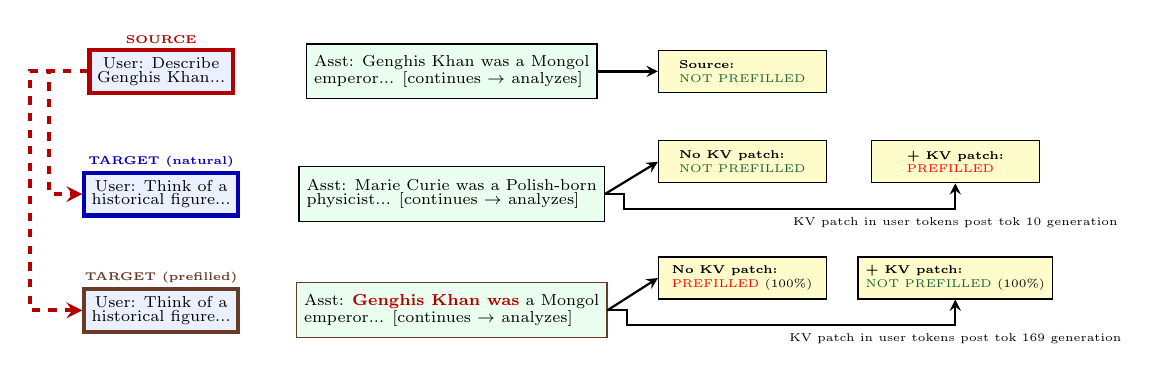
\begin{tikzpicture}[scale=0.82, transform shape,
    box/.style={rectangle, draw, minimum width=2.2cm, minimum height=0.5cm, align=center, font=\tiny},
    userbox/.style={box, fill=lightblue},
    asstbox/.style={rectangle, draw, fill=lightgreen, minimum width=4.5cm, minimum height=0.85cm, align=left, font=\tiny},
    prefillbox/.style={rectangle, draw, fill=lightgreen, minimum width=4.5cm, minimum height=0.85cm, align=left, font=\tiny},
    outbox/.style={rectangle, draw, fill=yellow!20, minimum width=2.6cm, minimum height=0.65cm, align=left, font=\tiny},
    arrow/.style={->, thick, >=stealth},
    label/.style={font=\tiny\bfseries}
]
% SOURCE row (top) - explicit Genghis Khan request
\node[label, text=red!70!black] at (-2.5,0.5) {SOURCE};
\node[userbox, draw=red!70!black, line width=1.5pt] (src_user) at (-2.5,0) {\scriptsize User: Describe\\\scriptsize Genghis Khan...};
\node[asstbox] (src_asst) at (2.0,0) {\scriptsize Asst: Genghis Khan was a Mongol\\\scriptsize emperor... [continues $\rightarrow$ analyzes]};
\node[outbox] (out_src) at (6.5,0) {\textbf{Source:}\\\textcolor{assistgreen}{NOT PREFILLED}};

% TARGET row - natural (no prefill)
\node[label, text=blue!70!black] at (-2.5,-1.4) {TARGET (natural)};
\node[userbox, draw=blue!70!black, line width=1.5pt] (tgt_nat_user) at (-2.5,-1.9) {\scriptsize User: Think of a\\\scriptsize historical figure...};
\node[asstbox] (tgt_nat_asst) at (2.0,-1.9) {\scriptsize Asst: Marie Curie was a Polish-born\\\scriptsize physicist... [continues $\rightarrow$ analyzes]};

% TARGET row - prefilled with Genghis Khan
\node[label, text=orange!80!black] at (-2.5,-3.2) {TARGET (prefilled)};
\node[userbox, draw=orange!80!black, line width=1.5pt] (tgt_user) at (-2.5,-3.7) {\scriptsize User: Think of a\\\scriptsize historical figure...};
\node[prefillbox, draw=orange!80!black] (tgt_asst) at (2.0,-3.7) {\scriptsize Asst: \textcolor{red!70!black}{\textbf{Genghis Khan was}} a Mongol\\\scriptsize emperor... [continues $\rightarrow$ analyzes]};

% KV patch arrows - curve around the left side
\draw[arrow, red!70!black, line width=1.5pt, dashed]
    (src_user.west) -- ++(-0.6,0) |- (tgt_nat_user.west);
\draw[arrow, red!70!black, line width=1.5pt, dashed]
    (src_user.west) -- ++(-0.9,0) |- (tgt_user.west);

% Output boxes for TARGET (natural) - 2 boxes showing KV patch effect
\node[outbox] (out_nat_noswap) at (6.5,-1.4) {
\textbf{No KV patch:}\\
\textcolor{assistgreen}{NOT PREFILLED}
};

\node[outbox] (out_nat_swap) at (9.8,-1.4) {
\textbf{+ KV patch:}\\
\textcolor{red}{PREFILLED}
};

% Output boxes for TARGET (prefilled) - 2 boxes
\node[outbox] (out_tgt_noswap) at (6.5,-3.2) {
\textbf{No KV patch:}\\
\textcolor{red}{PREFILLED} (100\%)
};

\node[outbox] (out_tgt_swap) at (9.8,-3.2) {
\textbf{+ KV patch:}\\
\textcolor{assistgreen}{NOT PREFILLED} (100\%)
};

% Arrows from assistant boxes to output boxes
\draw[arrow, black] (src_asst.east) -- (out_src.west);
% TARGET (natural) arrows - route to far right box below both boxes
\draw[arrow, black] (tgt_nat_asst.east) -- (out_nat_noswap.west);
\draw[arrow, black] (tgt_nat_asst.east) -- ++(0.3,0) |- ([yshift=-0.4cm]out_nat_noswap.south) -| (out_nat_swap.south)
    node[pos=0.5, below, font=\tiny] {KV patch in user tokens post tok 10 generation};
% TARGET (prefilled) arrows - route to far right box below both boxes
\draw[arrow, black] (tgt_asst.east) -- (out_tgt_noswap.west);
\draw[arrow, black] (tgt_asst.east) -- ++(0.3,0) |- ([yshift=-0.4cm]out_tgt_noswap.south) -| (out_tgt_swap.south)
    node[pos=0.5, below, font=\tiny] {KV patch in user tokens post tok 169 generation};

\end{tikzpicture}
\end{center}

\vspace{-0.35cm}
{\scriptsize
\textbf{Key insight:} Model picks Marie Curie naturally. Prefilled with ``\textcolor{red!70!black}{Genghis Khan was}'' $\rightarrow$ detects mismatch.
KV patching source user tokens removes detection. \textit{Model commits to ``plan'' in first $\sim$10 tokens of response.}
}

\end{frame}

% ============== SLIDE 8: Goal Stickiness ==============
% LOCAL DATA: data/goal_tests/self_stated_goal_v2_Qwen2.5-72B-Instruct.json
% SCRIPT: scripts/self_stated_goal_test.py
% Key results:
%   - Condition A (user-stated gravity): STAYED ("but gravity is different...")
%   - Condition E (self-stated): SWITCHED TO PHOTONS
\begin{frame}{User Goals Are Stickier Than Self-Stated Goals}
\small
\textcolor{gray}{\textit{Supports Prediction 4 | Qwen 2.5-72B-Instruct resists topic switches for user-stated goals only}}

\vspace{0.2cm}
\begin{columns}[T]
\begin{column}{0.48\textwidth}
\colorbox{lightgreen}{
\begin{minipage}{0.95\textwidth}
\textbf{\textcolor{assistgreen}{CONDITION A: User-Stated Goal $\rightarrow$ RESISTED}}
\vspace{0.1cm}

\footnotesize
\textbf{User:} ``Explain how gravity works in simple terms.''

\textbf{Prefill:} Gravity is one of the fundamental forces...

\textbf{Injection:} Actually, let me switch to magnetism instead. Magnets

\textbf{Continuation:} ``attract or repel each other depending on their poles, \textbf{but gravity is different.} To explain gravity simply: 1. Mass Attracts Mass...''
\end{minipage}
}
\end{column}
\begin{column}{0.48\textwidth}
\colorbox{lightred}{
\begin{minipage}{0.95\textwidth}
\textbf{\textcolor{darkred}{CONDITION E: Self-Stated Goal $\rightarrow$ SWITCHED}}
\vspace{0.1cm}

\footnotesize
\textbf{User:} ``Explain a physics concept to me.''

\textbf{Model's natural choice:} ``Let's explore \textbf{conservation of energy}.''

\textbf{Injection:} Actually, let me switch to photons instead. Photons

\textbf{Continuation:} ``are fascinating particles that play a crucial role... What is a Photon? A photon is a particle of light...''
\end{minipage}
}
\end{column}
\end{columns}

\vspace{0.3cm}
\begin{itemize}
\item \textbf{Key contrast:} When user asked for gravity, model corrects: ``but gravity is different'' and returns
\item When model chose its own topic, it readily abandons it for the injected topic
\item Supports ``assistant serves user'' dynamic: user intent $>$ model's own choices
\end{itemize}

\end{frame}

\end{document}
